\documentclass[]{article}
\usepackage{lmodern}
\usepackage{graphicx}
\usepackage{adjustbox}
\usepackage{amssymb,amsmath}
\usepackage{ifxetex,ifluatex}
\usepackage{listings}
\usepackage[T1]{fontenc}
\usepackage[utf8]{inputenc}
\usepackage{microtype}
\usepackage[margin=1in]{geometry}
\usepackage{hyperref}
\usepackage{framed}
\usepackage{graphicx,grffile}
\makeatletter
\def\maxwidth{\ifdim\Gin@nat@width>\linewidth\linewidth\else\Gin@nat@width\fi}
\def\maxheight{\ifdim\Gin@nat@height>\textheight\textheight\else\Gin@nat@height\fi}
\makeatother
% Scale images if necessary, so that they will not overflow the page
% margins by default, and it is still possible to overwrite the defaults
% using explicit options in \includegraphics[width, height, ...]{}
\setkeys{Gin}{width=\maxwidth,height=\maxheight,keepaspectratio}
\setlength{\parindent}{0pt}
\setlength{\parskip}{6pt plus 2pt minus 1pt}
\setlength{\emergencystretch}{3em}  % prevent overfull lines
\providecommand{\tightlist}{%
  \setlength{\itemsep}{0pt}\setlength{\parskip}{0pt}}

%%% Change title format to be more compact
\usepackage{titling}

% Create subtitle command for use in maketitle
\newcommand{\subtitle}[1]{
  \posttitle{
    \begin{center}\large#1\end{center}
    }
}

\setlength{\droptitle}{-2em}
  \title{MSAN 621 - Homework 1}
  \pretitle{\vspace{\droptitle}\centering\huge}
  \posttitle{\par}
  \author{Andre Guimaraes Duarte}
  \preauthor{\centering\large\emph}
  \postauthor{\par}
  \predate{\centering\large\emph}
  \postdate{\par}
  \date{October 31, 2016}
  
% Redefines (sub)paragraphs to behave more like section*s
\ifx\paragraph\undefined\else
\let\oldparagraph\paragraph
\renewcommand{\paragraph}[1]{\oldparagraph{#1}\mbox{}}
\fi
\ifx\subparagraph\undefined\else
\let\oldsubparagraph\subparagraph
\renewcommand{\subparagraph}[1]{\oldsubparagraph{#1}\mbox{}}
\fi

\usepackage{color}

%%%%%%%%%%%%%%%%%%%%%%%%%%%%%%%%%%%%%%%%%%%%%%%%%%%%%%%%%%%%%%%%%%%%%%%%%%%%%%%%%%%%%%%%%%%%%%%%%%%%%%%%%%%%%%%%%%%%%%%
\begin{document}
\maketitle

\section{The Boston Data Set}

The models are trained with all data except the last 50 rows, which are reserved to test the models' performance.

For SLR, we get an MSE of 10.967.

For kNN, we get an MSE that varies according to k, as shown in the table below:

\begin{tabular}{c|c}
k & MSE\\
\hline
1 & 29.299\\
2 & 24.532\\
3 & 22.003\\
4 & 25.754\\
5 & 26.200\\
6 & 24.441\\
7 & 24.615\\
8 & 22.820\\
9 & 24.117\\
10 & 22.371\\
11 & 23.036\\
12 & 24.953\\
13 & 23.774\\
14 & 24.388\\
15 & 27.162\\
16 & 25.311\\
17 & 24.743\\
18 & 25.761\\
19 & 27.539\\
20 & 27.362\\
\end{tabular}

Plotting MSE against k for both models, we get the image below:

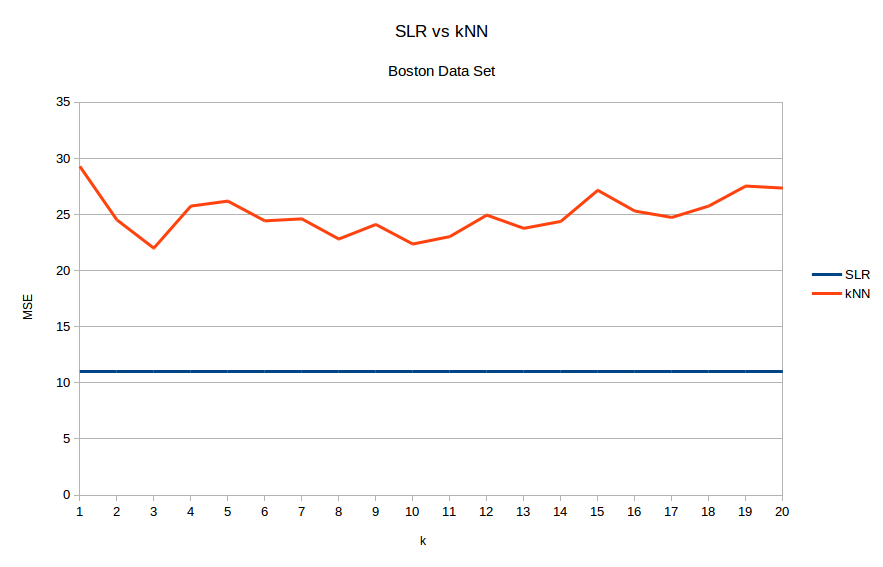
\includegraphics[width=\linewidth]{boston.png}

We can see that we get a lower test MSE with SLR than kNN, for any value of k. For this example, simple linear regression is a better algorithm for predicting new data from the Boston Data Set.

\section{The U.S. Monthly Climate Normals Data Set}


\end{document}
